\documentclass[french]{article}
\usepackage[T1]{fontenc}
\usepackage[utf8]{inputenc}
\usepackage{lmodern}
\usepackage[a4paper]{geometry}
\usepackage{babel}
\usepackage{listings}             % Include the listings-package
\usepackage{amsfonts}
\usepackage{color}
\usepackage{stmaryrd}

\usepackage{tikz}
\usepackage{tikz-qtree}

\definecolor{mygreen}{rgb}{0,0.6,0}
\definecolor{mygray}{rgb}{0.5,0.5,0.5}
\definecolor{mymauve}{rgb}{0.58,0,0.82}

\lstset{ %
  backgroundcolor=\color{white},   % choose the background color; you must add \usepackage{color} or \usepackage{xcolor}; should come as last argument
  basicstyle=\footnotesize,        % the size of the fonts that are used for the code
  breakatwhitespace=false,         % sets if automatic breaks should only happen at whitespace
  breaklines=true,                 % sets automatic line breaking
  captionpos=b,                    % sets the caption-position to bottom
  commentstyle=\color{mygreen},    % comment style
  deletekeywords={...},            % if you want to delete keywords from the given language
  escapeinside={\%*}{*)},          % if you want to add LaTeX within your code
  extendedchars=true,              % lets you use non-ASCII characters; for 8-bits encodings only, does not work with UTF-8
  frame=single,	                   % adds a frame around the code
  keepspaces=true,                 % keeps spaces in text, useful for keeping indentation of code (possibly needs columns=flexible)
  keywordstyle=\color{blue},       % keyword style
  language=Python,                 % the language of the code
  morekeywords={*,...},            % if you want to add more keywords to the set
  numbers=left,                    % where to put the line-numbers; possible values are (none, left, right)
  numbersep=5pt,                   % how far the line-numbers are from the code
  numberstyle=\tiny\color{mygray}, % the style that is used for the line-numbers
  rulecolor=\color{black},         % if not set, the frame-color may be changed on line-breaks within not-black text (e.g. comments (green here))
  showspaces=false,                % show spaces everywhere adding particular underscores; it overrides 'showstringspaces'
  showstringspaces=false,          % underline spaces within strings only
  showtabs=false,                  % show tabs within strings adding particular underscores
  stepnumber=2,                    % the step between two line-numbers. If it's 1, each line will be numbered
  stringstyle=\color{mymauve},     % string literal style
  tabsize=2,	                   % sets default tabsize to 2 spaces
  title=\lstname                   % show the filename of files included with \lstinputlisting; also try caption instead of title
}

\title{Recherche des structures secondaires d’une chaîne d’ADN\\
\large Projet 2I003}
%\title{Recherche des structures secondaires d’une chaîne d’ADN}
\author{LI Mengda, GE Zhichun}


\begin{document}
\lstset{language=Python}	

\maketitle

\section{Exercice 1}

\subsection{}
\label{subsec:q1}
Comme un nucléotide ne peut former une paire avec lui même, donc 

\begin{center}
$\forall i\in\{1,...,n\}, \quad S_{i,i} = \{\}$ et $ E_{i,i} = 0$
\par\end{center}

\subsection{}
\label{subsec:q2}

	\subsubsection{}
	Si ni i, ni j ne sont couplés dans S$_{i,j}$ , alors
	%{\centering S$_{i,j}$ = S$_{i+1,j-1}$\par}
	\begin{center}
	$S_{i,j} = S_{i+1,j-1}$ \quad $E_{i,j} = E_{i+1,j-1}$
	\par\end{center}

	\subsubsection{}
	Si j n'est pas couplée dans S$_{i,j}$ , alors
	\[
	S_{i,j} = S_{i,j-1} \quad E_{i,j} = E_{i,j-1}
	\]

	\subsubsection{}
	Si $\left(i,j\right)\in S_{i,j}$, alors
	\[
	S_{i,j}   = S_{i+1,j-1}\, \cup \, \left(i,j\right) \quad  E_{i,j} = E_{i+1,j-1}+ 1
	\]

	\subsubsection{}
	Si $\left(k,j\right)\in S_{i,j}$ avec $k\in\left\{ i+1,...,j-1\right\} $, alors
	\[
	S_{i,j}= S_{i,k-1}\cup S_{k,j} \quad E_{i,j} = E_{i,k-1} + E_{k,j} 
	\]
	car, par hypothèse, il n'existe pas de nœud: lorsqu'on coupe en k, on ne coupe pas de couple dans ce cas là, il n'y a donc pas de perte. Sinon, on a $S_{i,j} \subset S_{i,k-1}\cup S_{k,j} $ dans tous les cas.
\subsection{}
\label{subsec:q3}
	\subsubsection{}

		Par la question \ref{subsec:q2}, résumons en distinguant tous les cas possibles:
\\
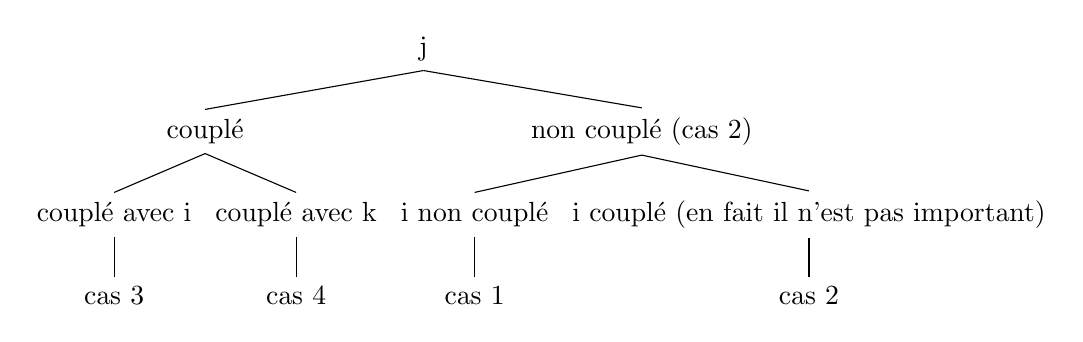
\begin{tikzpicture}
\Tree 
[.j	[.couplé 
			[.{couplé avec i} {cas 3} ]    [.{couplé avec k} {cas 4} ] 
	]
	[.{non couplé (cas 2)} 
			[.{i non couplé} {cas 1} ]	[.{i couplé (en fait il n'est pas important)} {cas 2} ]
	]
]

\end{tikzpicture}	
		\begin{enumerate}  
		\item \label{itm:1}
			 Soit ni i, ni j ne sont couplés dans S$_{i,j}$ , alors E$_{i,j}$ = E$_{i+1,j-1}$, \\
			et on a toujours E$_{i,j} \geq E_{i+1,j-1}$ dans tous les cas.
		\item Soit j n'est pas couplée dans S$_{i,j}$ , alors  E$_{i,j}$ = E$_{i,j-1}$, \\
			et on a toujours E$_{i,j} \geq E_{i,j-1}$ dans tous les cas.
	%	\item Soit i n'est pas couplée dans S$_{i,j}$ , alors  E$_{i,j}$ = E$_{i+1,j}$
		\item Soit j est couplé avec i, c'est à dire $\left(i,j\right)\in S_{i,j}$, alors E$_{i,j}$  = E$_{i+1,j-1}+1$
		\item Soit j est couplé avec un $k\in\left\{ i+1,...,j-1\right\} $, alors $E_{i,j} = E_{i,k-1} + E_{k,j}$,\\ sinon $E_{i,j} \geq E_{i,k-1} + E_{k,j}$ car $S_{i,j} \supset \, S_{i,k-1}\cup S_{k,j}\quad \forall k \in\left\{ i+1,...,j-1\right\}$
		\end{enumerate}
		
		Soit la fonction e :$ \{1, ... , n\} \times{} \{1, ... , n\} \rightarrow{} \{0, 1\}$ qui vaut 1 ssi i et j peuvent être couplés. \par
		\begin{description}
		\item
		\underline{Dans le cas  \ref{itm:1} et cas 3, $E_{i,j} = E_{i+1,j-1} + e(i,j)$ }  
et on a  \underline{$E_{i,j} \geq E_{i+1,j-1} + e(i,j)$ dans tous les cas. } 
			\begin{itemize} 
			\item si j est couplé avec i, $ e(i,j) = 1$, E$_{i,j}  = E_{i+1,j-1}+1 = E_{i+1,j-1}+ e(i,j) $, 
			\item sinon $ e(i,j) = 0$, on a toujours E$_{i,j} \geq E_{i+1,j-1} = E_{i+1,j-1}+ e(i,j)$ par le \ref{itm:1}.
			\end{itemize}	
		\item
		\underline{Dans le cas 2, $E_{i,j} = E_{i,j-1}$} et on a \underline{$E_{i,j} \geq E_{i,j-1}$ dans tous les cas.} car S$_{i,j} \supset S_{i,j-1}$
		\item
		Par le cas 4, $\forall k \in\left\{ i+1,...,j-1\right\} \; E_{i,j} \geq E_{i,k-1} + E_{k,j}$. Donc \underline{ $E_{i,j} \geq  \displaystyle \max_{i<k<j}  E_{i,k-1} + E_{k,j}$ dans tous les cas}.
		\\Et
		s'il existe $k_{0}\in\left\{ i+1,...,j-1\right\}$ tel que  $\left(k_{0},j\right)\in S_{i,j}$, $E_{i,j} = E_{i,k_{0}-1} + E_{k_{0},j}$\\
		Dans ce cas-là, le max est atteint:\\
		 $E_{i,k_{0}-1} + E_{k_{0},j} \geq  \displaystyle \max_{i<k<j}  E_{i,k-1} + E_{k,j}$ et $ \displaystyle \max_{i<k<j}  E_{i,k-1} + E_{k,j} \geq  E_{i,k_{0}-1} + E_{k_{0},j}$\\
		D'où \underline{ $E_{i,j} = E_{i,k_{0}-1} + E_{k_{0},j} = \displaystyle \max_{i<k<j}  E_{i,k-1} + E_{k,j}$ dans le cas 4}
		\end{description}
		En conclusion: $E_{i,j}$ est un majorant de l'ensemble $\{E_{i+1,j-1} + e(i,j), \, E_{i,j-1}, \,  \displaystyle \max_{i<k<j}  E_{i,k-1} \}$, et ce majorant est atteint: il y a toujours un cas où la condition d'égalité est vrai. 
		Donc
\begin{center}
 $E_{i,j} =\max\{E_{i+1,j-1} + e(i,j), \, E_{i,j-1}, \,  \displaystyle \max_{i<k<j}  E_{i,k-1} + E_{k,j}\}$
\par\end{center}
		...
	\subsubsection{}
	Si k = j, $ E_{k,j}=E_{j,j}=0$ par \ref{subsec:q1}, donc $E_{i,j-1}=(E_{i,j-1}+E_{j,j})\in \{E_{i,k-1} + E_{k,j} \mid i<k\leq j   \} $, et 
\begin{center}
$E_{i,j-1}\leq \max \{E_{i,k-1} + E_{k,j} \mid i<k\leq j   \} $
\par\end{center}

\begin{center}
On en déduit que $E_{i,j} =\max\{E_{i+1,j-1} + e(i,j), \,   \displaystyle \max_{i<k \leq j}  E_{i,k-1} + E_{k,j}\}$
\par\end{center}

\pagebreak
\subsection{Code en Python3}
\begin{lstlisting}[frame=single]  % Start your code-block

def tailleMaxRec(a: str, i: int, j: int) -> int:
    n= len(a)
    assert 1 <= i <= n and 1 <= j <= n, 'impossible de tronquer'
    
    if a == '' or i >= j:
        return 0

    def couple(i: int, j:int) -> bool:
        return {a[i-1], a[j-1]} in [ {'A','T'}, {'C','G'} ]
    
    def e(i: int, j: int) -> {0,1}:
        if couple(i,j):
            return 1
        else:
            return 0

    return max(tailleMaxRec(a, i+1, j-1) + e(i,j),
               max([tailleMaxRec(a, i, k-1) + tailleMaxRec(a, k, j)
                    for k in range(i+1, j+1)]) )
	\end{lstlisting}


\subsection{}
Cette fonction se termine car chaque fois on appelle récursivement sur une sous-partie de séquence [i+1, j-1], le début de sous-séquence i est strictement croissant et la fin de sous-séquence j est stricetement décroissante. Dans $\mathbb{N}$, l'ordre est bien fondé donc i, j se rencontre en certaine récursion. Lorsque i, j se rencontre, c'est à dire $i \leq j$, la fonction retourne une valeure et se termine en dépillant récursivement.
\par
Cette fonction calcule exactement $\max\{E_{i+1,j-1} + e(i,j), \,    \max_{i<k<j}  E_{i,k-1} + E_{k,j}\}$, elle est valide selon la question \ref{subsec:q3}.

\subsection{}
\subsubsection{}
Pour $u_{0}$, $(p = 0) \Rightarrow (i = j)$. Donc l'appel de fonction retourne simplement 0, $u_{0}=1$ \par
Pour $u_{1}$, $(p = 1) \Rightarrow (i + 1 = j)$, donc cet appel retourne 
\begin{lstlisting}
max(tailleMaxRec(a, i+1, j-1) + e(i,j),
               max([tailleMaxRec(a, i, k-1) + tailleMaxRec(a, k, j)
                    for k in range(i+1, j+1)]) )\end{lstlisting}
Vu que i + 1 = j,  tailleMaxRec(a, i+1, j-1) retourne simplement 0 car $i+1=j\geq j-1$.\\
Analysons la dernière itérable 
\begin{lstlisting}
[tailleMaxRec(a, i, k-1) + tailleMaxRec(a, k, j) for k in range(i+1, j+1)]\end{lstlisting}
range(j ,j+1) ne contient que j, donc cette liste n'a qu'un élément, cela vaut dire qu'on appelle deux fois  \lstinline{tailleMaxRec}.
En sommant, $u_{1} = 3$
\subsubsection{}

Soit $p \leq 2$, pour $u_{p}$\\
	\begin{itemize}
	\item
	On appelle d'abord une fois la fonction elle-même: \lstinline{tailleMaxRec(a, i, j)}, on a 1 appel. 
	\item
	Et puis on appelle  \lstinline{ tailleMaxRec (a, i+1, j-1) },\\
	 $(j-1)-(i+1)=(j-i)-2=0$, on a donc $u_{0}$ appel(s).
	\item
	Enfin, pour\\
 \lstinline{[ tailleMaxRec(a,i,k-1) + tailleMaxRec(a,k,j) for k in range(i+1, j+1) ]}\\
	\lstinline{range(i+1, j+1)} équivaut à $\llbracket i+1, i+p \rrbracket$, car p = j - i, j = i + p\\
Le nombre d'appel de \lstinline{tailleMaxRec(a, i, k-1)} équivaut $u_{k-1-i}$,\\Le nombre d'appel de \lstinline{tailleMaxRec(a, k, j)} équivaut $u_{p+i-k}$\\	
On a donc $\sum_{k=i+1}^{i+p} u_{k-1-i} + \sum_{k=i+1}^{i+p} u_{p+i-k}$ d'appels.\\
Pour la première, en éffectuant un changement de variable q = k- (i+1), on a bien $\sum_{q=0}^{p-1} u_{q}$\\
Pour la deuxième, en éffectuant un changement de variable q = p + i - k, on a  $\sum_{q=p-1}^{0} u_{q}$ qui vaut en effet $\sum_{q=0}^{p-1} u_{q}$.\\
En sommant les deux sommes, on a bien $2\sum_{i=0}^{p-1} u_{i}$
	\end{itemize}
\par
En conclusion, $u_{p}=u_{0}+1+2\sum_{i=0}^{p-1} u_{i}$

\subsubsection{}
Démontrons par récurrence $u_{n} \geq 2^n$.
	\begin{itemize}
	\item 
	Cas de base, $u_{0}=1 \geq 2^0$,  $u_{1} = 3 \geq 2^1$ vérifié dans question 1.\\ Et $u_{2}=u_{0} +1+2(u_{0}+u_{1}) = 10 \geq 2^2$
	\item
	Induction: par récurrence forte\\
Soit $n \in \mathbb{N}, n\geq2 $ fixé, supposons on a $u_{k} \geq 2^k \; \forall k \in \{2, ..., n\}$\\
$u_{n+1}=u_{0}+1+2\sum_{i=0}^{n} u_{i} \geq 2^0 +2^0 + 2\sum_{i=0}^{n} 2^i = 2^1 + 2\frac{1-2^{n+1}}{1-2} = 2^{n+2}  \geq 2^{n+1}$

	\end{itemize}
\par
En conclusion, $\forall n \in \mathbb{N}, \; u_{n}  \geq 2^n$

\subsubsection{}
On en déduit que sa complexité est de $\mathcal{O}(2^n)$

\subsection{}
Sa complexité est de $\Theta(n^3)$.\\
Il y a une boucle for simple et une boucle for triplé dans cet algorithme. Le reste est de temps constant.\\
La première boule fait (n-1) itération. Dans chaque itération on éffectue un nombre constant d'opérations. Donc il est de complexité $\Theta(n)$.\\
Le cœur de l'analyse est au sein de la deuxième boule composé en effet de trois boucle for, voici le code Python qui l'implémente:
\begin{lstlisting}
    for p in range(1, n):
        for i in range(1, n-p+1):
            E[(i,i+p)] = max( E[(i+1,i+p-1)] + e(a, i, i+p),
                             max ( E[(i,k-1)] + E[(k,i+p)]
                                  for k in range(i+1, i+p+1)))
\end{lstlisting}
Il fait en effet $\sum_{p=1}^{n-1}\sum_{i=1}^{n-p}\sum_{k=i+1}^{i+p}$ itérations dans laquelle on effectue un nombre fini d'opération.\\
$\sum_{p=1}^{n-1}\sum_{i=1}^{n-p}\sum_{k=i+1}^{i+p}=\sum_{p=1}^{n-1}\sum_{i=1}^{n-p}\frac{(i+1+i+p)p}{2}=\sum_{p=1}^{n-1}\frac{( \frac{(3+p)p}{2} + \frac{(2(n-p) + 1 + p)p}{2}) (n-p)}{2}$\\
$\Leftrightarrow \frac{
(\frac{( \frac{(3+1)1}{2} + \frac{(2(n-1) + 1 + 1)1}{2}) (n-1)}{2} + 
\frac{( \frac{(3+(n-1))(n-1)}{2} + \frac{(2(n-(n-1)) + 1 + (n-1))(n-1)}{2}) (n-(n-1))}{2})(n-1)}
{2}$\\
$\Leftrightarrow \frac{
(\frac{( n + \frac{3}{2}) (n-1)}{2} + 
\frac{( \frac{(n+2)(n-1)}{2} + \frac{(n+2)(n-1)}{2}) }{2})(n-1)}
{2}$
$\Leftrightarrow \frac{
(\frac{n^2 +  n/2 - 3/2}{2} + 
\frac{n^2 + n - 2}{2})(n-1)}
{2}$
$\Leftrightarrow \frac{
(2n^2 + 3n/2 - 7/2)(n-1)}
{4}$\\
$\Leftrightarrow \frac{
(4n+7)(n-1)(n-1)}
{8} \in \Theta(n^3) $

\section{Exercice 2}
\subsection{Code en Python3}
\begin{lstlisting}
a = 'TCGGCTGCATTTCGA'
def e(a: str, i: int, j: int) -> {0,1}:
    """Retourner 1 si i,j sont couples, 0 sinon."""
    def couple(a: str, i: int, j:int) -> bool:
        return {a[i-1], a[j-1]} in [ {'A','T'}, {'C','G'} ]

    if couple(a,i,j):
        return 1
    else:
        return 0
def tailleMaxRec(a: str, i: int, j: int) -> int:
    n= len(a)
    assert 1 <= i <= n and 1 <= j <= n, 'impossible de tronquer'
    if a == '' or i >= j:
        return 0
    return max(tailleMaxRec(a, i+1, j-1) + e(a,i,j),
               max([tailleMaxRec(a, i, k-1) + tailleMaxRec(a, k, j)
                    for k in range(i+1, j+1)]) )

def tailleMaxIter(a: str, i: int, j: int) -> int:
    n= len(a)
    E=dict()
    E[(1,1)] = 0
    for i in range(2, n+1):
        E[(i,i)] = 0
        E[(i,i-1)] = 0
    for p in range(1, n):
        for i in range(1, n-p+1):
            E[(i,i+p)] = max( E[(i+1,i+p-1)] + e(a, i, i+p),
                             max ( E[(i,k-1)] + E[(k,i+p)]
                                  for k in range(i+1, i+p+1)))
    return E[(i,j)]

if __name__ == '__main__':
    import timeit
    print("E_3_13 calcule par l'algorithme recursive =", tailleMaxRec(a, 3, 13))
    print("E_3_13 calcule par l'algorithme iterative =", tailleMaxIter(a, 3, 13))
    print('10 executions de la fonction recursive prennent',
          timeit.timeit("tailleMaxRec(a, 3, 13)", number=10,
                        setup="from __main__ import tailleMaxRec, a"),'secondes')
    print('10 executions de la fonction iterative prennent',
          timeit.timeit("tailleMaxIter(a, 3, 13)", number=10,
                        setup="from __main__ import tailleMaxIter, a"),'secondes')

\end{lstlisting}
Le résultat de teste donne
\begin{lstlisting}
E_3_13 calcule par l'algorithme recursive = 4
E_3_13 calcule par l'algorithme iterative = 4
10 executions de la fonction recursive prennent 1.213047794000886 secondes
10 executions de la fonction iterative prennent 0.004673413001000881 secondes
\end{lstlisting}

\subsection{}
\begin{lstlisting}
from random import randrange 

def SeqAleatoire(n: int) -> str:
    return ''.join(['A','T','C','G'][randrange(4)] for i in range(n))
\end{lstlisting}
Quelques testes:
\begin{lstlisting}
>>> SeqAleatoire (10)
'TAGACCATAG'
>>> SeqAleatoire (10)
'TCGACAGATT'
>>> SeqAleatoire (11)
'GGGGTGGGGCT'
>>> SeqAleatoire (11)
'CTTAATTCTGG'
\end{lstlisting}

\subsection{Test expérimental: question 3, 4, 5}
\begin{lstlisting}
import timeit

def testRec() -> None:
    n = 1
    lt0 = 0
    while True:
        a = SeqAleatoire(n)
        t1 = timeit.timeit("tailleMaxRec(a, 1, n)", number=1,
                        setup="from __main__ import tailleMaxRec",
                           globals=locals())
        print('''CRec({0:d})  = {1:7f}, log'(CRec({0:d})) = {2:7f}'''.format(
            n, t1, log(t1) - lt0))
        print()
        if t1 > 600: 
            break
        n = n + 1
        lt0 = log(t1)
\end{lstlisting}
\pagebreak
\begin{lstlisting}
def testIter() -> None:
    n = 1
    while True:
        a = SeqAleatoire(n)
        t2 = timeit.timeit("tailleMaxIter(a, 1, n)", number=1,
                setup="from __main__ import tailleMaxIter",
                   globals=locals())
        print('CIter({0:d}) = {1:7f}, CIter({0:d})/{0:d}^3 = {2:7f}'.format(
            n, t2, t2 / n**3))
        print()
        if t2 > 300: 
            break
        n = n + 1

\end{lstlisting}

\subsubsection{Test de la fonction récursive}
\begin{lstlisting}
>>> testRec()
CRec(1)  = 0.000003, log'(CRec(1)) = -12.782327

CRec(2)  = 0.000085, log'(CRec(2)) = 3.406688

CRec(3)  = 0.000040, log'(CRec(3)) = -0.739755

CRec(4)  = 0.000066, log'(CRec(4)) = 0.490493

CRec(5)  = 0.000169, log'(CRec(5)) = 0.939710

CRec(6)  = 0.000681, log'(CRec(6)) = 1.392812

CRec(7)  = 0.002577, log'(CRec(7)) = 1.331125

CRec(8)  = 0.006125, log'(CRec(8)) = 0.865912

CRec(9)  = 0.015648, log'(CRec(9)) = 0.937961

CRec(10)  = 0.041903, log'(CRec(10)) = 0.984977

CRec(11)  = 0.129540, log'(CRec(11)) = 1.128638

CRec(12)  = 0.408717, log'(CRec(12)) = 1.149034

CRec(13)  = 1.262126, log'(CRec(13)) = 1.127531

CRec(14)  = 4.076094, log'(CRec(14)) = 1.172342

CRec(15)  = 13.468090, log'(CRec(15)) = 1.195184

CRec(16)  = 43.075104, log'(CRec(16)) = 1.162622

CRec(17)  = 144.504570, log'(CRec(17)) = 1.210366

CRec(18)  = 480.611199, log'(CRec(18)) = 1.201747

CRec(19)  = 1446.607645, log'(CRec(19)) = 1.102334

\end{lstlisting}
On peut voir que le temps d'execution de tailleMaxRec croît très vite en raison de sa complexité exponentielle. Lorsque n = 18, cela prend plus de 5 minutes pour exécuter et plus de 10 minutes lorsque n = 19. Donc la plus grande valeur de n que je peux traiter est 19.\\
La pente de la droite $\log' CRec(n) \approx 1$, qui vaut dire que cette fonction est affine à n.

\subsubsection{Test de la fonction itérative}
Le calcul par l'itération est très efficace donc la plus grande valeur que je peux tester est relativement très grande et pratiquement je ne peux pas afficher le résultat de test entier. Je donne un extrait de test ici. On peut voir que $\frac{CIter(n)}{n^3}$ vaut constamment prèsque nul.
\begin{lstlisting}
CIter(1) = 0.000005, CIter(1)/1^3 =  0.000005

CIter(2) = 0.000040, CIter(2)/2^3 =  0.000005

CIter(3) = 0.000028, CIter(3)/3^3 =  0.000001

...

CIter(25) = 0.001586, CIter(25)/25^3 =  0.000000

CIter(26) = 0.001813, CIter(26)/26^3 =  0.000000

CIter(27) = 0.001995, CIter(27)/27^3 =  0.000000

CIter(28) = 0.002584, CIter(28)/28^3 =  0.000000

...

CIter(72) = 0.025478, CIter(72)/72^3 =  0.000000

CIter(73) = 0.026434, CIter(73)/73^3 =  0.000000

CIter(74) = 0.028332, CIter(74)/74^3 =  0.000000

CIter(75) = 0.029268, CIter(75)/75^3 =  0.000000

...

CIter(100) = 0.062157, CIter(100)/100^3 =  0.000000

CIter(101) = 0.065108, CIter(101)/101^3 =  0.000000

CIter(102) = 0.069097, CIter(102)/102^3 =  0.000000

...

CIter(200) = 0.467661, CIter(200)/200^3 =  0.000000

CIter(201) = 0.470119, CIter(201)/201^3 =  0.000000

CIter(202) = 0.517451, CIter(202)/202^3 =  0.000000

CIter(203) = 0.469706, CIter(203)/203^3 =  0.000000
...
CIter(300) = 2.228376, CIter(300)/300^3 =  0.000000

CIter(301) = 2.223427, CIter(301)/301^3 =  0.000000...
\end{lstlisting}
Voici quelques recherche à la main pour trouver <la plus grande valeur>. Lorsque n = 1500, cela prend déjà plus de 5 min pour calculer. Donc je choisis 1500 comme <la plus grande valeur>.
\begin{lstlisting}
>>> n=500
>>> timeit.timeit("tailleMaxIter(SeqAleatoire(n), 1, n)", number=1,
                setup="from __main__ import tailleMaxIter",
                   globals=globals())
15.326990880996163
>>> n = 700
>>> timeit.timeit("tailleMaxIter(SeqAleatoire(n), 1, n)", number=1,
                setup="from __main__ import tailleMaxIter",
                   globals=globals())
39.779907284995716
>>> n = 1000
>>> timeit.timeit("tailleMaxIter(SeqAleatoire(n), 1, n)", number=1,
                setup="from __main__ import tailleMaxIter",
                   globals=globals())
126.6036247910015
>>> n = 1500
>>> timeit.timeit("tailleMaxIter(SeqAleatoire(n), 1, n)", number=1,
                setup="from __main__ import tailleMaxIter",
                   globals=globals())
468.63339252900187
\end{lstlisting}

\pagebreak
\section*{Appendice}
On peut ajouter une comparaison de $\frac{CIter(n)}{n^2}$ pour voir la complexité expérimentalement: $\frac{CIter(n)}{n^2}$ est en fait croissant!\par Donc il n'est pas possible que la complexité de l'algorithme itérative soit de $\Theta(n^2)$.
\begin{lstlisting}
CIter(1) = 0.000005, CIter(1)/1^3 = 0.000005, CIter(1)/1^2 = 0.000005

CIter(2) = 0.000028, CIter(2)/2^3 = 0.000004, CIter(2)/2^2 = 0.000007

CIter(3) = 0.000130, CIter(3)/3^3 = 0.000005, CIter(3)/3^2 = 0.000014

CIter(4) = 0.000057, CIter(4)/4^3 = 0.000001, CIter(4)/4^2 = 0.000004

...

CIter(100) = 0.071538, CIter(100)/100^3 = 0.000000, CIter(100)/100^2 = 0.000007

CIter(101) = 0.068498, CIter(101)/101^3 = 0.000000, CIter(101)/101^2 = 0.000007

CIter(102) = 0.067363, CIter(102)/102^3 = 0.000000, CIter(102)/102^2 = 0.000006

...

CIter(198) = 0.446628, CIter(198)/198^3 = 0.000000, CIter(198)/198^2 = 0.000011

CIter(199) = 0.462426, CIter(199)/199^3 = 0.000000, CIter(199)/199^2 = 0.000012

CIter(200) = 0.470033, CIter(200)/200^3 = 0.000000, CIter(200)/200^2 = 0.000012

...

CIter(250) = 1.016588, CIter(250)/250^3 = 0.000000, CIter(250)/250^2 = 0.000016

CIter(251) = 1.017460, CIter(251)/251^3 = 0.000000, CIter(251)/251^2 = 0.000016

CIter(252) = 1.049520, CIter(252)/252^3 = 0.000000, CIter(252)/252^2 = 0.000017

...

CIter(268) = 1.318201, CIter(268)/268^3 = 0.000000, CIter(268)/268^2 = 0.000018

CIter(269) = 1.327808, CIter(269)/269^3 = 0.000000, CIter(269)/269^2 = 0.000018

CIter(270) = 1.354491, CIter(270)/270^3 = 0.000000, CIter(270)/270^2 = 0.000019

CIter(271) = 1.368608, CIter(271)/271^3 = 0.000000, CIter(271)/271^2 = 0.000019

...

CIter(287) = 1.682067, CIter(287)/287^3 = 0.000000, CIter(287)/287^2 = 0.000020

CIter(288) = 1.745375, CIter(288)/288^3 = 0.000000, CIter(288)/288^2 = 0.000021

...

CIter(299) = 2.005110, CIter(299)/299^3 = 0.000000, CIter(299)/299^2 = 0.000022

CIter(300) = 2.021642, CIter(300)/300^3 = 0.000000, CIter(300)/300^2 = 0.000022

CIter(301) = 2.101834, CIter(301)/301^3 = 0.000000, CIter(301)/301^2 = 0.000023

CIter(302) = 2.104127, CIter(302)/302^3 = 0.000000, CIter(302)/302^2 = 0.000023

...

CIter(347) = 3.612243, CIter(347)/347^3 = 0.000000, CIter(347)/347^2 = 0.000030

CIter(348) = 3.701992, CIter(348)/348^3 = 0.000000, CIter(348)/348^2 = 0.000031

CIter(349) = 3.754785, CIter(349)/349^3 = 0.000000, CIter(349)/349^2 = 0.000031

...

CIter(400) = 6.285140, CIter(400)/400^3 = 0.000000, CIter(400)/400^2 = 0.000039

CIter(401) = 6.664165, CIter(401)/401^3 = 0.000000, CIter(401)/401^2 = 0.000041

CIter(402) = 7.256984, CIter(402)/402^3 = 0.000000, CIter(402)/402^2 = 0.000045

CIter(403) = 6.513025, CIter(403)/403^3 = 0.000000, CIter(403)/403^2 = 0.000040

CIter(404) = 6.679665, CIter(404)/404^3 = 0.000000, CIter(404)/404^2 = 0.000041

...

CIter(424) = 8.426929, CIter(424)/424^3 = 0.000000, CIter(424)/424^2 = 0.000047

CIter(425) = 8.165203, CIter(425)/425^3 = 0.000000, CIter(425)/425^2 = 0.000045

CIter(426) = 7.977312, CIter(426)/426^3 = 0.000000, CIter(426)/426^2 = 0.000044

CIter(427) = 8.363914, CIter(427)/427^3 = 0.000000, CIter(427)/427^2 = 0.000046

CIter(428) = 8.285690, CIter(428)/428^3 = 0.000000, CIter(428)/428^2 = 0.000045

\end{lstlisting}
\end{document}
























Induction:
Soit $n \in \mathbb{N}, n\geq2 $ fixé, supposons $u_{n} = u_{0} + 1 + 2\sum_{i=0}^{1} u_{i}$
supposons $u_{k} = u_{k-2} + 1 + 2\sum_{i=0}^{k-1} u_{i}$
Démontrons par récurrence  le nombre d'appel de cette partie vaut $2\sum_{i=0}^{p-1} u_{i}$
		\begin{itemize}
		\item 
		Cas de base, p = 2, \lstinline{range(i+1, j+1)} équivaut à $\llbracket i+1, i+2 \rrbracket$, j = i +2
			\begin{description}
			\item
			Lorsque k = i + 1,\\
			on appelle \lstinline{tailleMaxRec(a, i, i)}, on a $u_{0}$ appel(s) et \\
			on appelle \lstinline{tailleMaxRec(a, i + 1, i + 2)}, on a $u_{1}$ appel(s)
			\item
			Lorsque k = i + 2,\\
			on appelle \lstinline{tailleMaxRec(a, i, i + 1)}, on a $u_{1}$ appel(s) et \\
			on appelle \lstinline{tailleMaxRec(a, i + 2, i + 2)}, on a $u_{0}$ appel(s)
			\end{description}
		On a bien  $ 2\sum_{i=0}^{1} u_{i}$ appels. \\\par
		\item
		Induction: Soit $n \in \mathbb{N}, n\geq2 $ fixé, supposons on a $2\sum_{i=0}^{n-1} u_{i}$ appels en $\llbracket i+1, i+n \rrbracket$ lorsque p = n. Notons P(n) le nombre d'appel sur $\llbracket i+1, i+n \rrbracket$.\\
Lorsque p = n + 1, $\llbracket i+1, i+n+1 \rrbracket= \llbracket i+1, i+n \rrbracket \cup \{n+1\}$, donc \begin{center} P(n+1) = P(n) + le nombre d'appel lorsque k = n+1 \end{center}	
		Lorsque k = n + 1,\\
		on appelle \lstinline{tailleMaxRec(a, i, n)}, on a $u_{n-i}$ appel(s) et \\
		on appelle \lstinline{tailleMaxRec(a, n + 1, i + n + 2)}, on a $u_{i+2}$ appel(s)	

	\end{itemize}